% % % % % % % % % % % % % % % % % % % % % % % % % % % % % % % %
% begin module approximate integration trapezoid-ex2
\begin{frame}
%\frametitle{Use the Trapezoidal Rule to approximate
%$\ds\int_0^\pi\sin(x)\; dx $.}




\begin{example}[Use the Trapezoidal Rule to approximate
$\ds\int_0^\pi\sin(x)\; dx$.  Compare your answers for $ n=4 $ and $ n=8$]
\[
 T_n=\frac{\Delta x}2\left[f(x_0)+2f(x_1)+2f(x_2)+\dots +2f(x_{n-1})\right]
\]
\begin{columns}[c]
  \begin{column}[t]{.6\textwidth}
\uncover<2->{
For $ n=4 $ we have $ \Delta x = \frac{b-a}{n}= \frac{\pi-0}{4}= \frac{\pi}{4}.$
} 
\uncover<3->{So
{\small
\begin{align*}
 T_4 & = \frac{\pi}{8}\left(f(0)+ 2f(\frac{\pi}{4}) + 2f(\frac{\pi}{2})+ 2f(\frac{3\pi}{4})+  f(\pi) \right)\\
 & = \frac{\pi}{8}\left(\sin(0)+ 2\sin\frac{\pi}{4} + 2\sin\frac{\pi}{2}+ 2\sin\frac{3\pi}{4}+  \sin\pi \right)\\
 \uncover<4->{&= \frac{\pi}{8}(0+\sqrt{2}+2+\sqrt{2}+0)=\frac{\pi(1+\sqrt{2})}{4}\\ & \approx 1.896
 }
\end{align*}
} %
} %

  \end{column}
  \begin{column}[t]{.4\textwidth}
\uncover<2->{
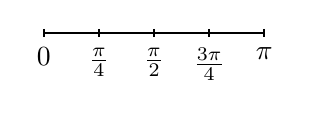
\begin{tikzpicture}[scale=.7]
\draw[thick] (0,0) -- (4,0) ; %edit here for the axis
\foreach \x in  {0,1,2,3,4} % edit here for the vertical lines
\draw[thick, shift={(\x,0)},color=black] (0pt,2pt) -- (0pt,-2pt);
\foreach \n/\texto in {0/{0},1/{\frac{\pi}{4}},2/{\frac{\pi}{2}},3/{\frac{3\pi}{4}},4/{\pi}}
\node[below] at (\n,-.1) {$\texto$};
\end{tikzpicture}
}

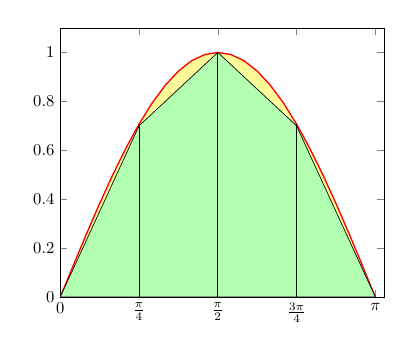
\begin{tikzpicture}[scale=.6]
  \begin{axis}[
    %grid=both,
    ymin=0,
    xmin=0,xmax=185,
    xtick={0,45,90,135,180},
        xticklabels={$0$, $\frac{\pi}{4}$,$ \frac{\pi}{2} $,$\frac{3\pi}{4}$, $ \pi $},
    ]
    \addplot[draw=none, domain=0:180,fill=yellow!40] {sin(x)}\closedcycle;
    \addplot[solid,thick,red,domain=0:180] {sin(x)};
\only<2->{     \addplot[fill=green!30,mark=none] coordinates {
           (0,0)
           (45,0.7)
           (90,1)
           (135,0.7)
           (180 ,0)
           (0,0)
           }; 
           \foreach \x in {45,90, 135}
           \addplot[mark=black] coordinates {
           (\x,0)
           (\x, {sin(\x)})
           (\x,0)
           };
}             
  \end{axis}
 

\end{tikzpicture}

%\includegraphics[width=\linewidth]{../../modules/approximate-integration/pictures/Tex2}\\
%\vspace*{1cm} 

%\uncover<5->{
%\includegraphics[width=\linewidth]{../../modules/approximate-integration/pictures/Tex3}\\
%}   
  \end{column}
\end{columns}


\end{example}

\end{frame}
% % % % % % % % % % % % % % % % % % % % % % % % % % % % % % % %
% % % % % % % % % % % % % % % % % % % % % % % % % % % % % % % %
\begin{frame}
%\frametitle{Use the Trapezoidal Rule to approximate
%$\ds\int_0^\pi\sin(x)\; dx $.}




\begin{example}[Use the Trapezoidal Rule to approximate
$\ds\int_0^\pi\sin(x)\; dx$.  Compare your answers for $ n=4 $ and $ n=8$]
\[
 T_n=\frac{\Delta x}2\left[f(x_0)+2f(x_1)+2f(x_2)+\dots +2f(x_{n-1})\right]
\]
\begin{columns}[c]
  \begin{column}{.6\textwidth}
\uncover<2->{
For $ n=8 $ we have $ \Delta x = \frac{\pi-0}{8}= \frac{\pi}{8}.   $
} 
\uncover<3->{So
{\small
\begin{align*}
T_8  = & \frac{\pi}{16}\left(\sin(0)+ 2\sin\frac{\pi}{8} + 2\sin\frac{\pi}{4}+ 2\sin\frac{3\pi}{8}+ 2\sin\frac{\pi}{2}\right.\\
& \left.+ 2\sin\frac{5\pi}{8}+ 2\sin\frac{3\pi}{4}+ 2\sin\frac{7\pi}{8}+ 2\sin\pi \right)\\
\uncover<4->{ &= \frac{\pi}{16}\left(2+2\sqrt{2}+4\sin\frac{\pi}{8}+4 \sin\frac{3\pi}{8}\right)\\ & \approx 1.974
 }
\end{align*}
} %
} %
  \end{column}
  \begin{column}{.4\textwidth}
\uncover<2->{
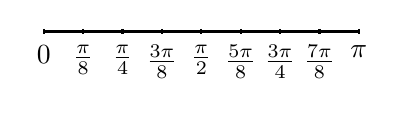
\begin{tikzpicture}[scale=.5]
\draw[thick] (0,0) -- (8,0) ; %edit here for the axis
\foreach \x in  {0,1,2,3,4,5,6,7,8} % edit here for the vertical lines
\draw[thick, shift={(\x,0)},color=black] (0pt,2pt) -- (0pt,-2pt);
\foreach \n/\texto in {0/{0},1/{\frac{\pi}{8}},2/{\frac{\pi}{4}},3/{\frac{3\pi}{8}},4/{\frac{\pi}{2}},5/{\frac{5\pi}{8}},6/{\frac{3\pi}{4}},7/{\frac{7\pi}{8}} ,8/{\pi}}
\node[below] at (\n,-.1) {$\texto$};
\end{tikzpicture}
}

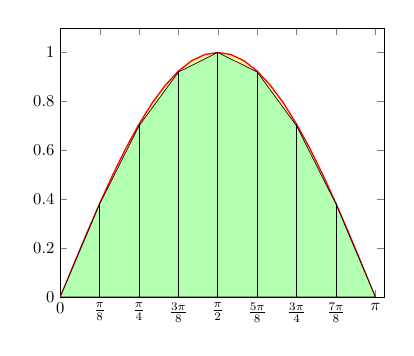
\begin{tikzpicture}[scale=.6]
  \begin{axis}[
    %grid=both,
    ymin=0,
    xmin=0,xmax=185,
    xtick={0,22.5,45,67.5, 90,112.5, 135,157.5, 180},
        xticklabels={$0$,$\frac{\pi}{8}$,$ \frac{\pi}{4} $,$\frac{3\pi}{8}$, $\frac{\pi}{2}$,$ \frac{5\pi}{8} $,$\frac{3\pi}{4}$,$\frac{7\pi}{8}$, $ \pi $},
    ]
    \addplot[draw=none, domain=0:180,fill=yellow!40] {sin(x)}\closedcycle;
    \addplot[solid,thick,red,domain=0:180] {sin(x)};
\only<2->{     \addplot[fill=green!30,mark=none] coordinates {
           (0,0)
           (22.5, 0.38)
           (45,0.7)
           (67.5,0.92)
           (90,1)
           (112.5,0.92)
           (135,0.7)
           (157.5,0.38)
           (180 ,0)
           (0,0)
           };
\foreach \x in {22.5,45,67.5, 90,112.5, 135,157.5}
\addplot[mark=black] coordinates {
(\x,0)
(\x, {sin(\x)})
(\x,0)
}; 
}
  \end{axis}


\end{tikzpicture}

%\includegraphics[width=\linewidth]{../../modules/approximate-integration/pictures/Tex2}\\
%\vspace*{1cm} 
%}
%\uncover<5->{
%\includegraphics[width=\linewidth]{../../modules/approximate-integration/pictures/Tex3}\\
%}   
  \end{column}
\end{columns}


\end{example}

\end{frame}
% % % % % % % % % % % % % % % % % % % % % % % % % % % % % % % %
% end module approximate integration trapezoid-ex2